\documentclass[10pt, a4paper]{memoir}

\usepackage[utf8]{inputenc}
\usepackage[T1]{fontenc}
\usepackage[polish]{babel}

\usepackage{graphicx}
\usepackage{caption}
\usepackage{verse}

\pagestyle{plain}
\linespread{1.3}

\setsecnumdepth{none}

\title{Po makale.}
\author{Kate Malec}
\date{\the\year}

\begin{document}

\maketitle
\newpage

\thispagestyle{empty}
\vspace*{\fill}
\begin{flushright}
    \itshape
    Z gorącymi pozdrowieniami
\end{flushright}
\vfill

\newpage
\tableofcontents
\newpage

% --- WIERSZE ---

\section{Życzenie}
\begin{verse}
Razu pewnego gnana arogancją\\
na pół złożoną kartkę\\
podałam sekretarce.![\vspace{\baselineskip}]

Chciałam rodzaj ludzki poznać,\\
zrozumieć istnienie.\\
W opisie ceny wpisałam \\
\textit{bez znaczenia}.![\vspace{\baselineskip}]

Teraz na pewno zrozumienia mam więcej,\\
że moje życie też kruche, a koszt przewyższa\\
zdolność kredytową serca.![\vspace{\baselineskip}]

Niestety, rubryki z cennikiem nie zmienię.\\
Staram się dalej rozumieć, jak zawsze,\\
a serce? Wymienię.
\end{verse}

\newpage
\section{Udało się}
\begin{verse}
Udało się,\\
dopieliście swego.\\
Lecz nie jestem pewna,\\
Naprawdę wiecie?\\
Chcecie tego?![\vspace{\baselineskip}]

Teraz już za późno,\\
serce upuściłam\\
po raz kolejny.\\
Potłukło się w mak drobny,\\
lecz komu to dzisiaj organ\\
potrzebny?![\vspace{\baselineskip}]

Teraz już bez uczuć,\\
tak, jak uczyliście,\\
idę przez życie,\\
a nowe wyrywam jak chwastu liście.![\vspace{\baselineskip}]

Rozum, tak jak serce,\\
roztrzaskała myśl ostra\\
jak skała.\\
I to nie jedna.\\
Człowiekiem poległam.![\vspace{\baselineskip}]

Teraz idę już sama dzielnie przez życie,\\
a wy sobie gratulujcie\\
zmiany dziecka w czarownicę.
\end{verse}

\newpage
\section{Szczapy}
\begin{verse}
Mój mąż gustuje w wieszakach\\
Niestety, ja nigdy nie byłam zbyt dobra\\
W byciu szczapą.![\vspace{\baselineskip}]

Martwiąc się o to zgubiłam dwa cale.\\
Może powiesi mąż na mnie oko,\\
gdy zrzucę jeszcze kawałek?![\vspace{\baselineskip}]

Nie można męża obwiniać,\\
Facet ma dobre geny.\\
A ja? no cóż, ja jestem przeciętna...\\
I nie po drodze mi do bycia cienką.
\end{verse}

\newpage
\begin{figure}[h]
    \centering
    % Wyśrodkowanie obrazu szerszego niż szerokość kolumny tekstu
    \makebox[\textwidth]{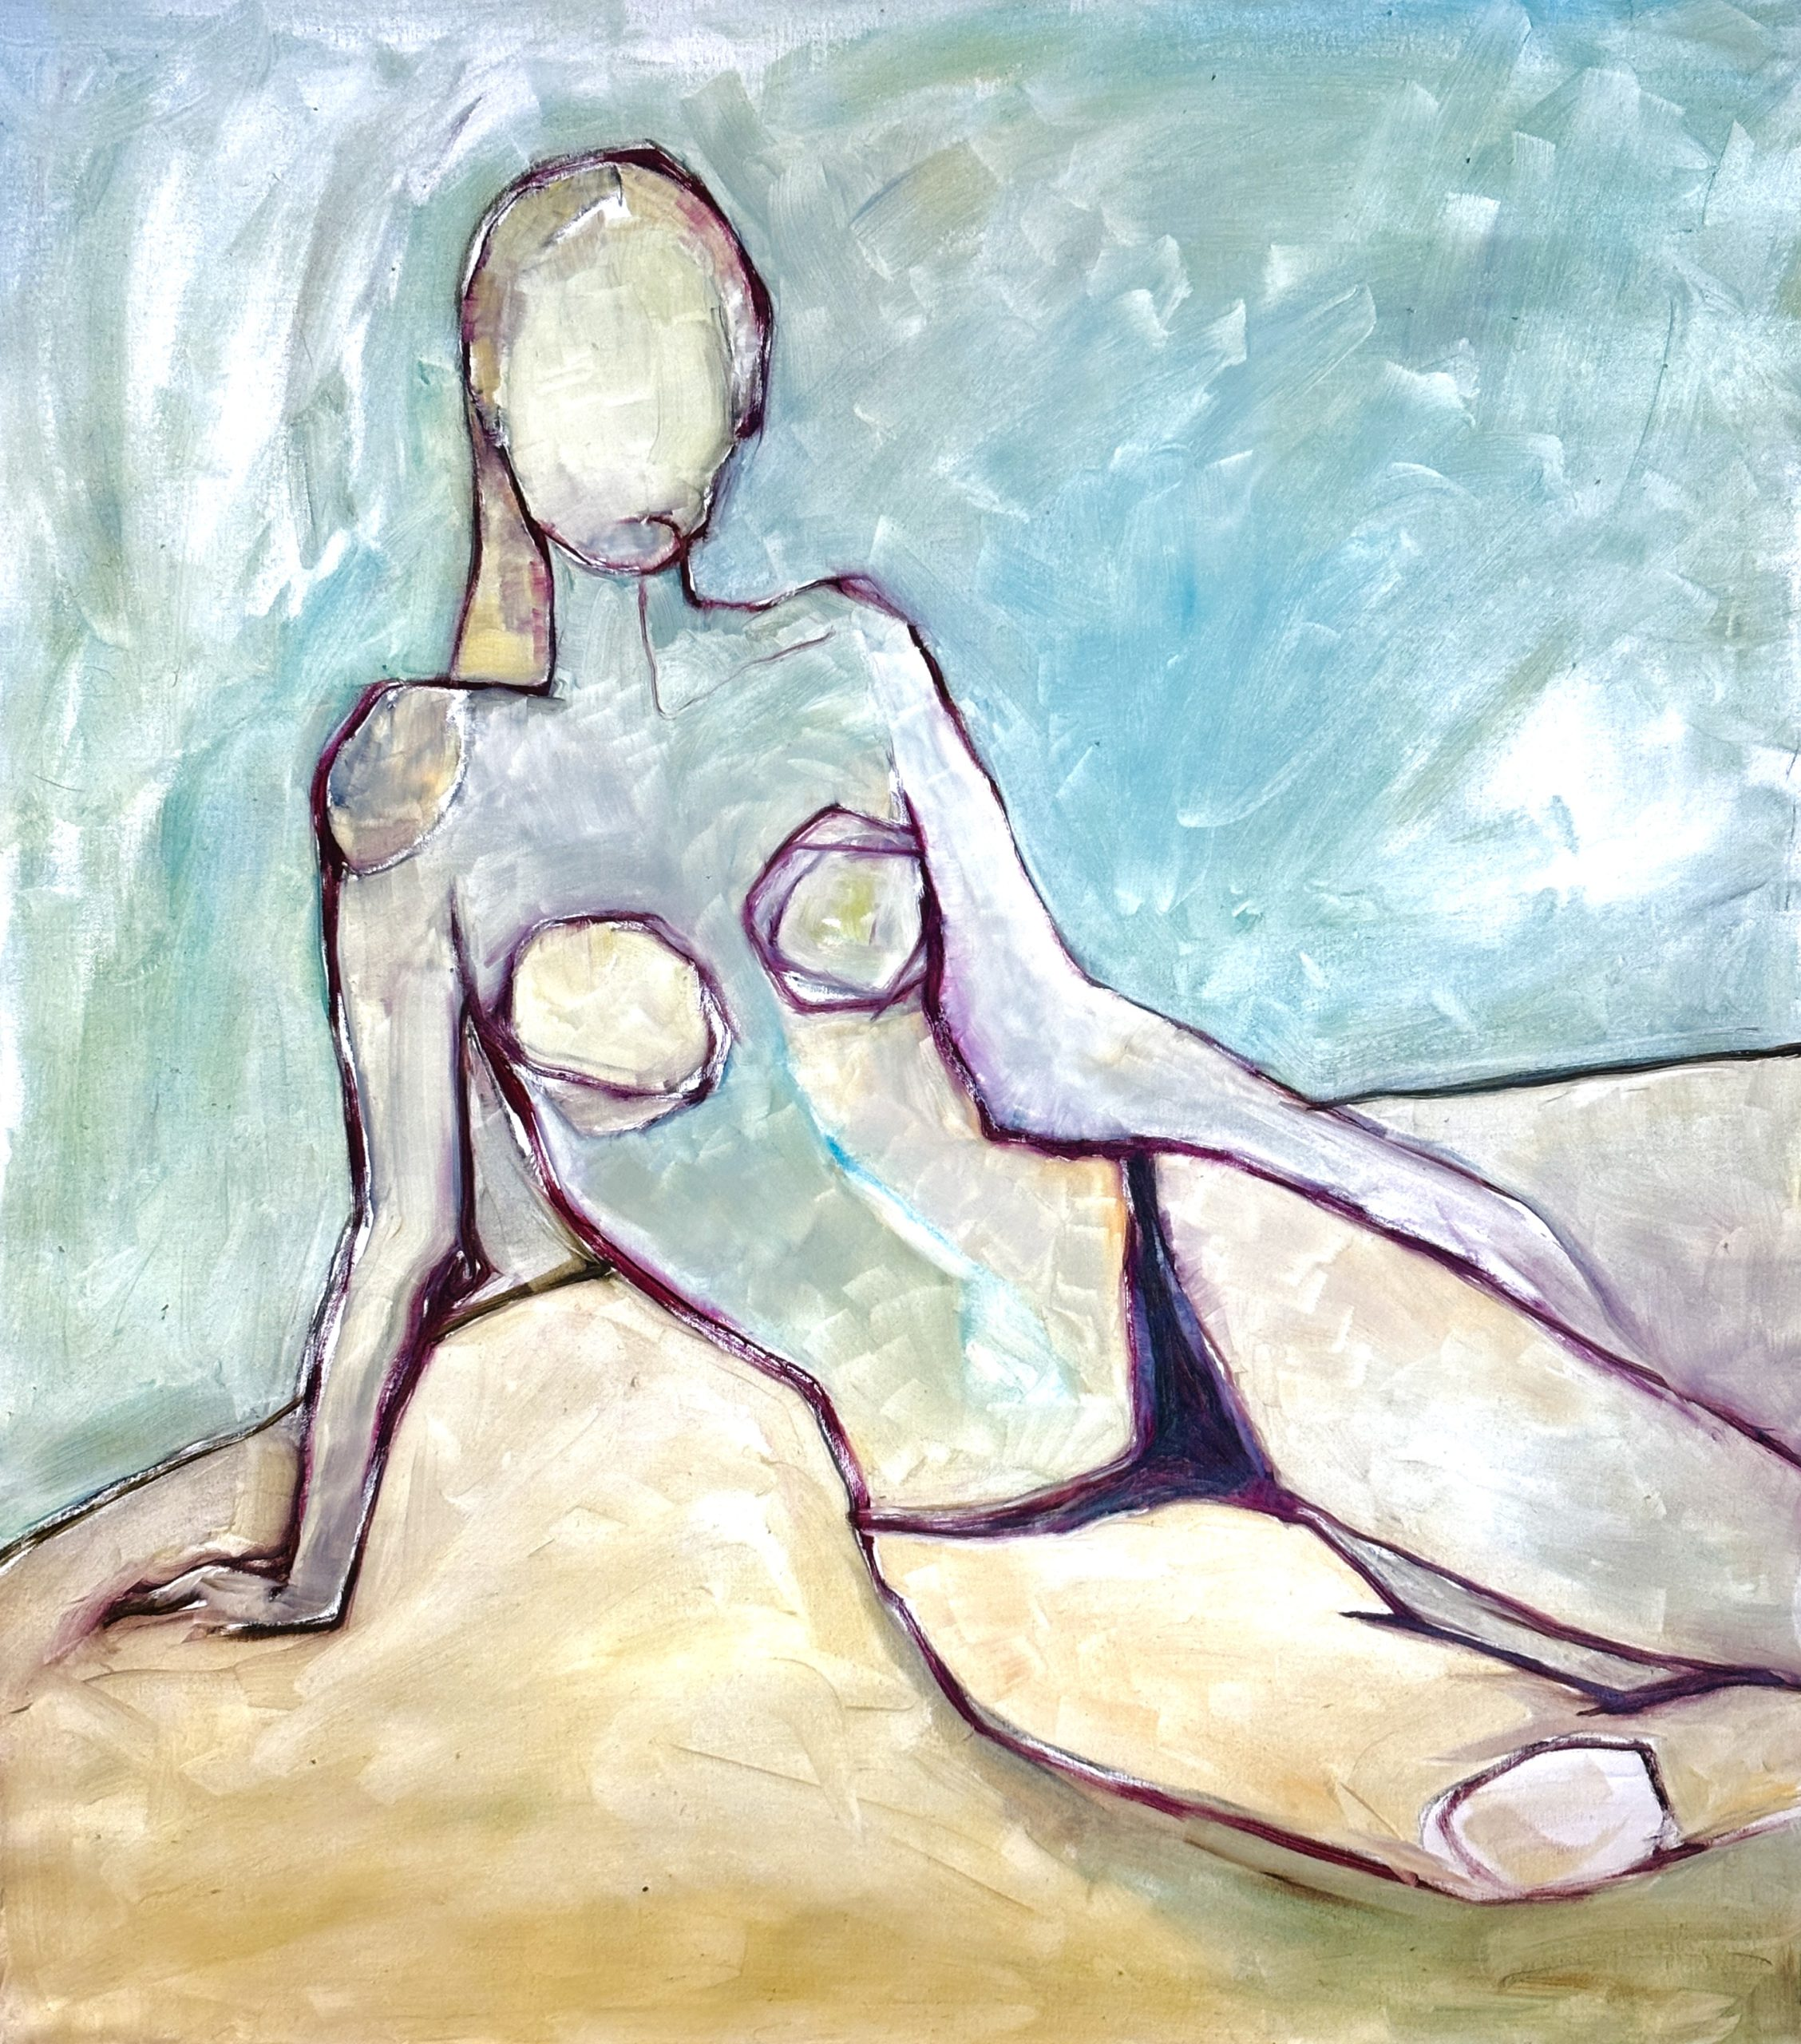
\includegraphics[width=1.1\textwidth]{img/szczapy-1.jpeg}}
    \caption*{Szczapy I, 80/70 cm, Oil on canvas, 2023}
\end{figure}

\newpage
\section{Cienka aż szczęka}
\begin{verse}
Moja matka -- ona to bywa cienka,\\
Lecz powód tego odmienny;\\
Dziadek o twardej szczęce\\
Wpędził niechcący \\
za dziecka mamę\\
w anoreksję.
\end{verse}

\newpage
\begin{figure}[h]
    \centering
    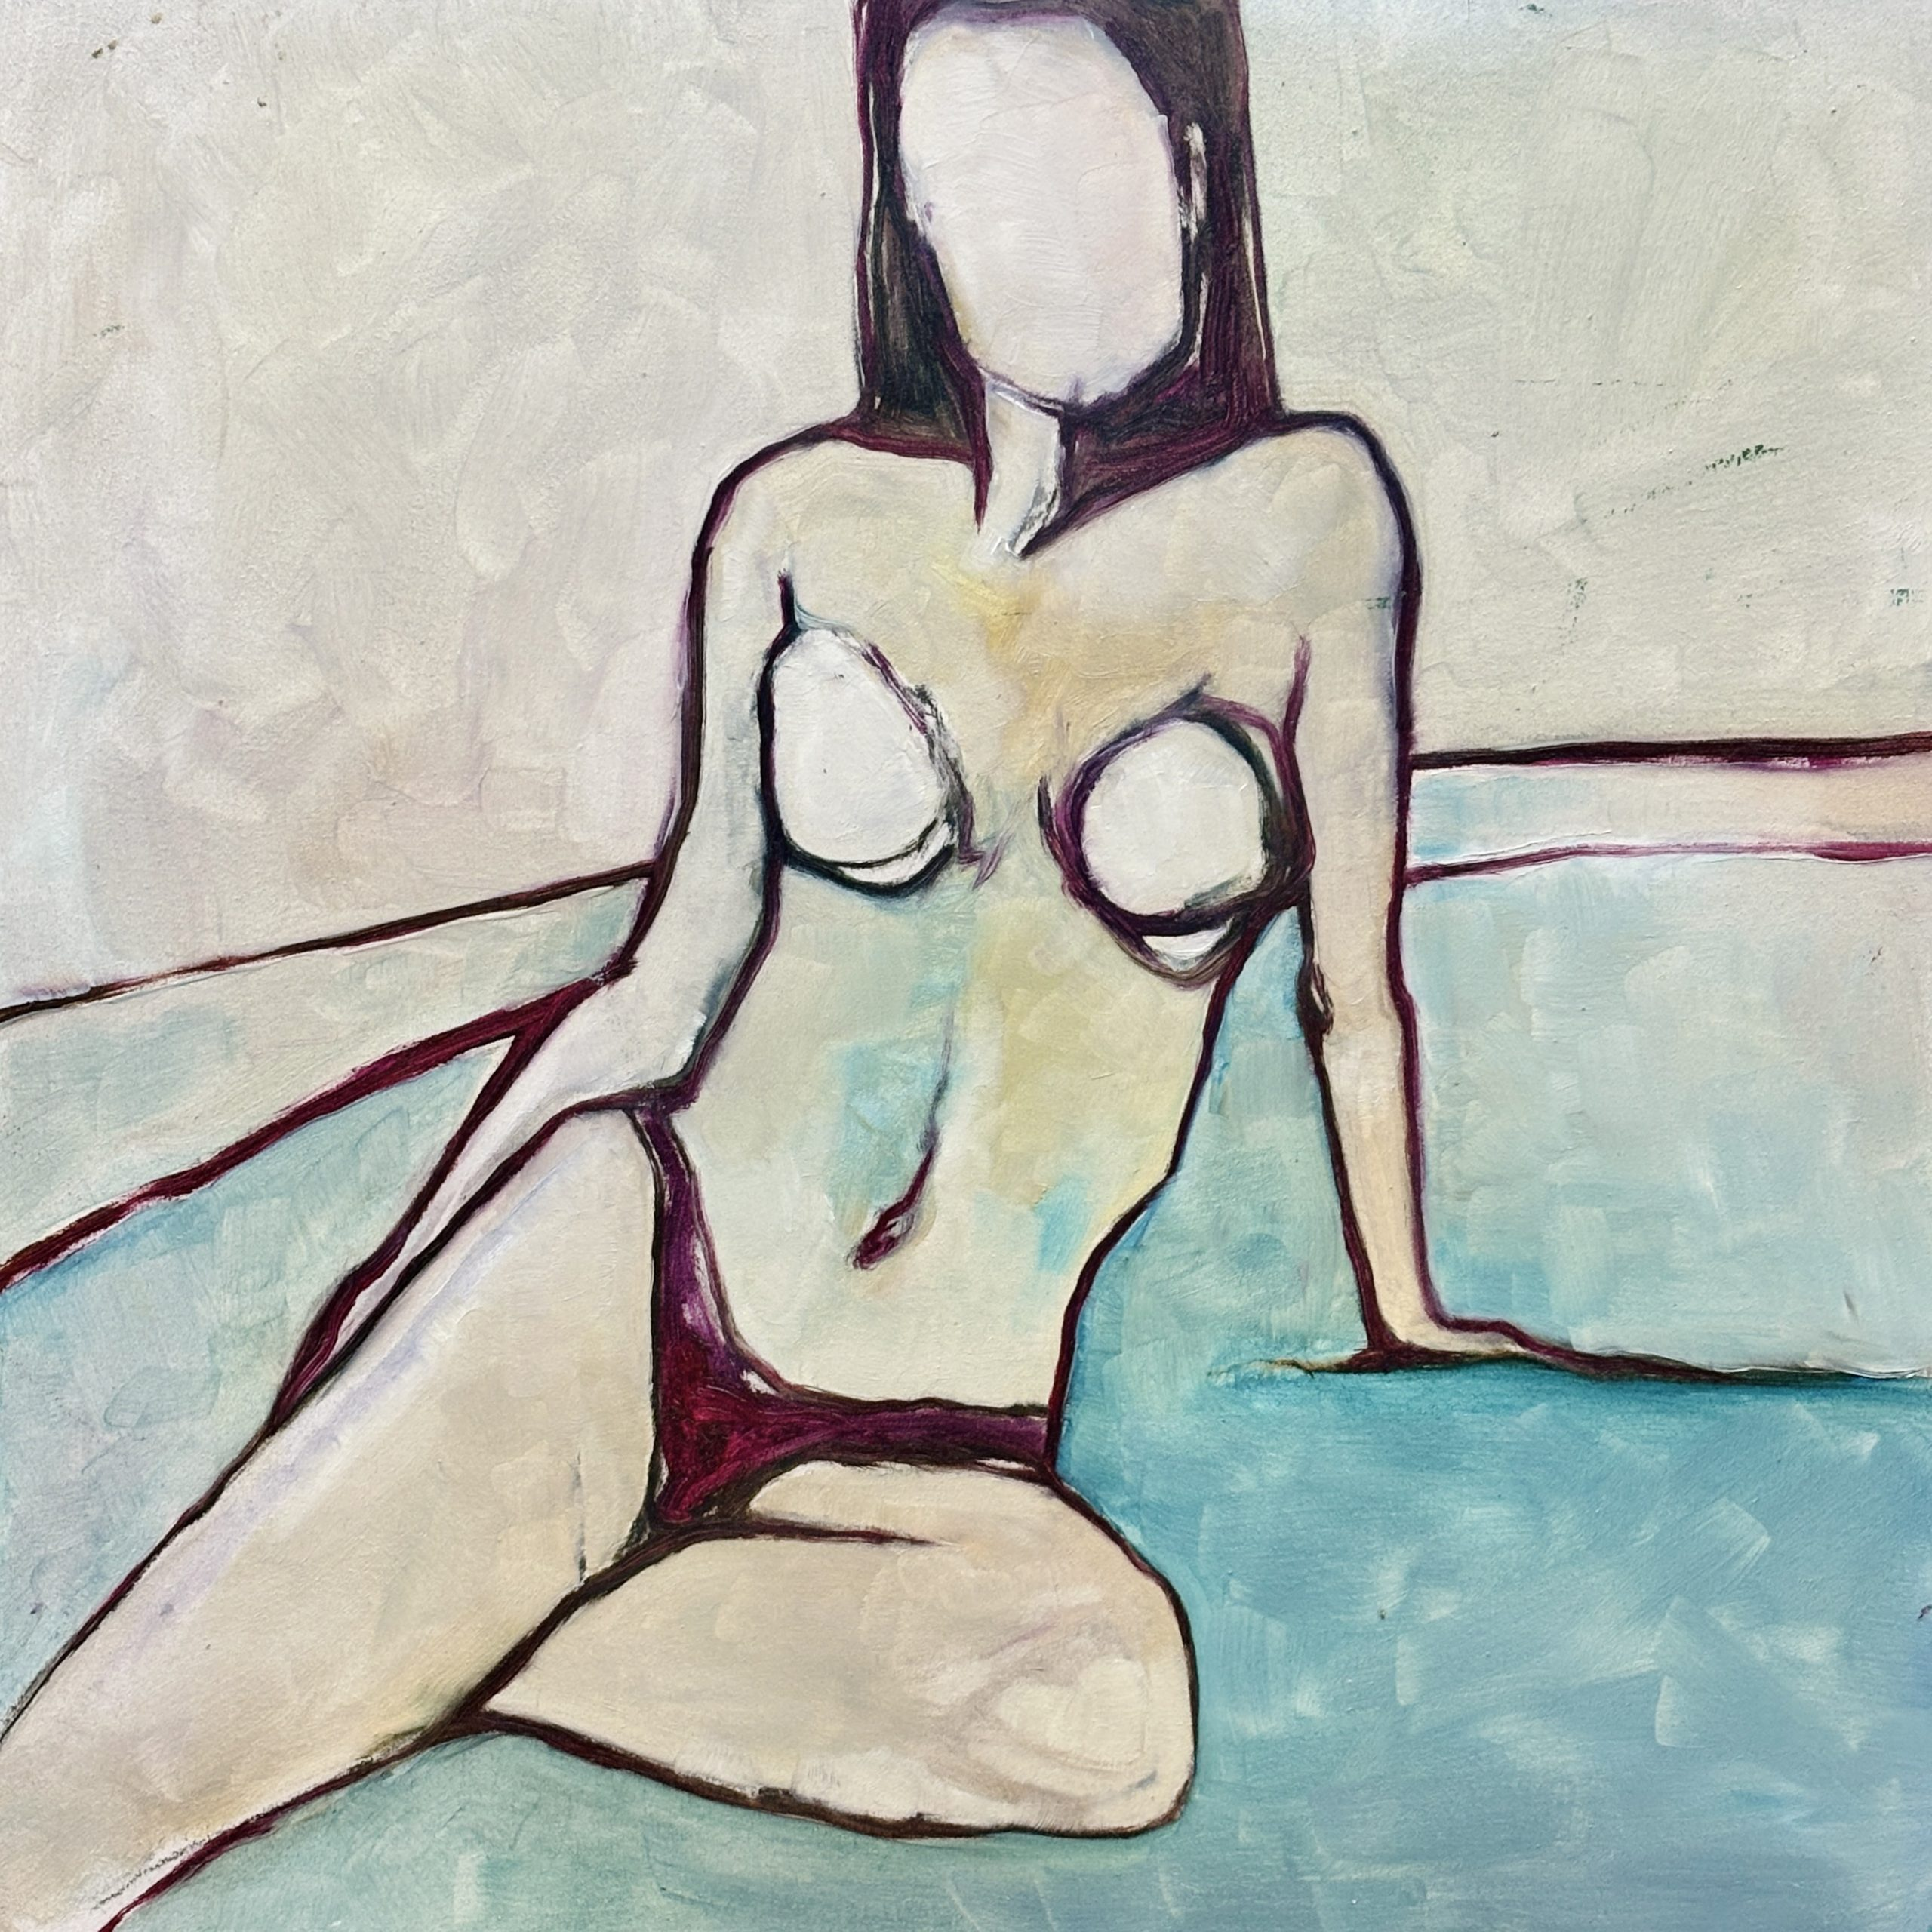
\includegraphics[width=0.9\textwidth]{img/szczapy-2.jpeg}
    \caption*{Szczapy II, 50/50 cm, Oil on canvas, 2023}
\end{figure}

\newpage
\section{Nowa runda}
\begin{verse}
Dzwonek\\
nowa runda wybiła\\
na ringu się spotkamy\\
czy opuściła siła?![\vspace{\baselineskip}]

Ja niestety nie mam wyboru\\
Na ringu stawić się muszę\\
inaczej z góry popiołem\\
obsypią moją duszę.![\vspace{\baselineskip}]

Tak, rozumiem\\
trzeba odpoczywać\\
lecz nie moja to wina,\\
walkirią się urodziłam.
\end{verse}

\end{document}